% Diagram 3/3 — Postgres schema (Drizzle ORM over Supabase, via Hyperdrive)
% Workflow -> workflow.tex   ·   Storage -> storage.tex
% Build:  pdflatex database.tex
\documentclass[border=14pt]{standalone}
\usepackage[T1]{fontenc}
\usepackage{lmodern}
\usepackage{tikz}
\usetikzlibrary{positioning, arrows.meta, shapes.geometric, backgrounds, fit, calc}

\definecolor{dbGreen}{HTML}{2E6F40}
\definecolor{dbGreenBg}{HTML}{E5F2E8}
\definecolor{wkBlue}{HTML}{1D4E89}
\definecolor{qOrange}{HTML}{C75B12}
\definecolor{stTeal}{HTML}{0E6B6B}
\definecolor{inkGray}{HTML}{475569}
\definecolor{todoGray}{HTML}{6B7280}

\newcommand{\pk}[1]{\textbf{#1}\,{\scriptsize\textcolor{qOrange}{PK}}}
\newcommand{\fk}[1]{#1\,{\scriptsize\textcolor{wkBlue}{FK}}}
\newcommand{\sub}[1]{{\scriptsize\textcolor{inkGray}{#1}}}
\newcommand{\tname}[1]{{\bfseries\color{dbGreen}#1}}

\begin{document}
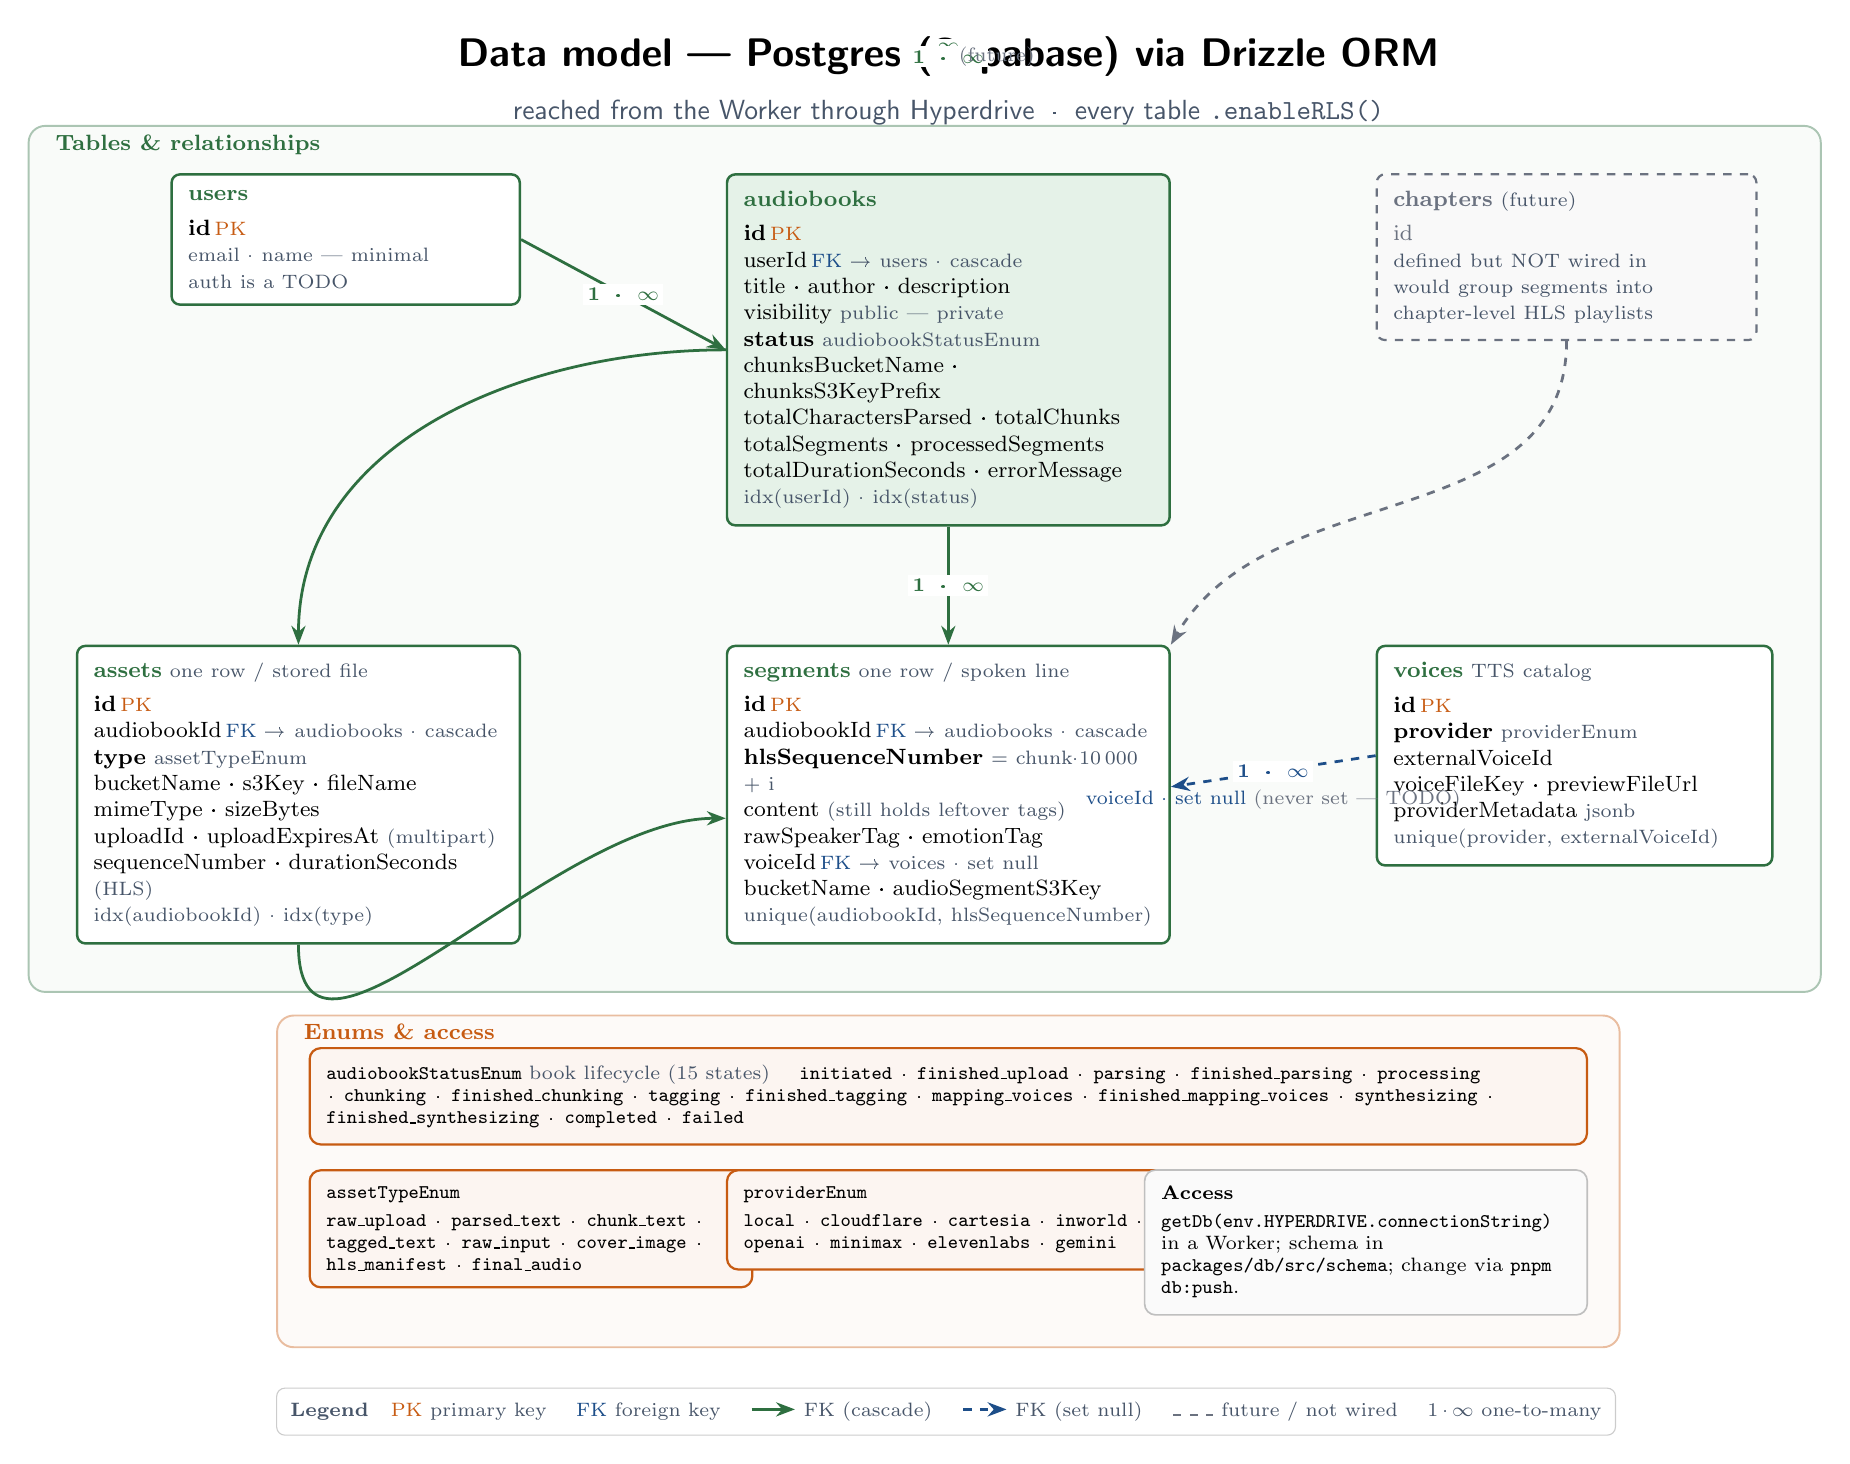
\begin{tikzpicture}[
  font=\sffamily,
  >={Stealth[length=2.6mm]},
  tbl/.style={rectangle, rounded corners=3pt, draw=dbGreen, line width=0.9pt,
              fill=white, align=left, inner sep=6pt, font=\footnotesize, text width=52mm},
  futuretbl/.style={rectangle, rounded corners=3pt, draw=todoGray, dashed, line width=0.8pt,
              fill=gray!5, align=left, inner sep=6pt, font=\footnotesize, text=todoGray, text width=44mm},
  enumbox/.style={rectangle, rounded corners=4pt, draw=qOrange, line width=0.8pt,
              fill=qOrange!6, align=left, inner sep=6pt, font=\scriptsize},
  note/.style={rectangle, rounded corners=4pt, draw=gray!50, line width=0.6pt,
              fill=gray!4, align=left, inner sep=6pt, font=\scriptsize},
  rel/.style={-{Stealth[length=2.4mm]}, line width=1pt, draw=dbGreen},
  relnull/.style={-{Stealth[length=2.4mm]}, line width=1pt, draw=wkBlue, dashed},
  card/.style={font=\scriptsize\bfseries, text=dbGreen, inner sep=1.5pt, fill=white},
]

% ===== Title =================================================================
\node[font=\sffamily\bfseries\Large] (title) {Data model — Postgres (Supabase) via Drizzle ORM};
\node[below=0.5mm of title, font=\sffamily, text=inkGray]
  {reached from the Worker through Hyperdrive \;·\; every table \texttt{.enableRLS()}};

% ===== Top row: users · audiobooks · chapters ===============================
\node[tbl, fill=dbGreenBg, below=11mm of title.south] (ab)
  {\tname{audiobooks}\\[3pt]
   \pk{id}\\
   \fk{userId} \sub{→ users · cascade}\\
   title · author · description\\
   visibility \sub{public | private}\\
   \textbf{status} \sub{audiobookStatusEnum}\\
   chunksBucketName · chunksS3KeyPrefix\\
   totalCharactersParsed · totalChunks\\
   totalSegments · processedSegments\\
   totalDurationSeconds · errorMessage\\
   \sub{idx(userId) · idx(status)}};

\node[tbl, text width=40mm] (users) at ($(ab.north west)+(-26mm,0)$) [anchor=north east]
  {\tname{users}\\[3pt]
   \pk{id}\\
   \sub{email · name — minimal}\\
   \sub{auth is a TODO}};

\node[futuretbl] (chap) at ($(ab.north east)+(26mm,0)$) [anchor=north west]
  {\textbf{chapters} \sub{(future)}\\[3pt]
   id\\
   \sub{defined but NOT wired in}\\
   \sub{would group segments into}\\
   \sub{chapter-level HLS playlists}};

% ===== Bottom row: assets · segments · voices ===============================
\node[tbl] (seg) at ($(ab.south)+(0,-15mm)$) [anchor=north]
  {\tname{segments} \sub{one row / spoken line}\\[3pt]
   \pk{id}\\
   \fk{audiobookId} \sub{→ audiobooks · cascade}\\
   \textbf{hlsSequenceNumber} \sub{= chunk·10\,000 + i}\\
   content \sub{(still holds leftover tags)}\\
   rawSpeakerTag · emotionTag\\
   \fk{voiceId} \sub{→ voices · set null}\\
   bucketName · audioSegmentS3Key\\
   \sub{unique(audiobookId, hlsSequenceNumber)}};

\node[tbl] (assets) at ($(seg.north west)+(-26mm,0)$) [anchor=north east]
  {\tname{assets} \sub{one row / stored file}\\[3pt]
   \pk{id}\\
   \fk{audiobookId} \sub{→ audiobooks · cascade}\\
   \textbf{type} \sub{assetTypeEnum}\\
   bucketName · s3Key · fileName\\
   mimeType · sizeBytes\\
   uploadId · uploadExpiresAt \sub{(multipart)}\\
   sequenceNumber · durationSeconds \sub{(HLS)}\\
   \sub{idx(audiobookId) · idx(type)}};

\node[tbl, text width=46mm] (voices) at ($(seg.north east)+(26mm,0)$) [anchor=north west]
  {\tname{voices} \sub{TTS catalog}\\[3pt]
   \pk{id}\\
   \textbf{provider} \sub{providerEnum}\\
   externalVoiceId\\
   voiceFileKey · previewFileUrl\\
   providerMetadata \sub{jsonb}\\
   \sub{unique(provider, externalVoiceId)}};

% ===== Relationships ========================================================
\draw[rel] (users.east) -- (ab.west)
  node[card, pos=0.5]{1 \;·\; $\infty$};
\draw[rel] (ab.south) -- (seg.north)
  node[card, pos=0.5]{1 \;·\; $\infty$};
\draw[rel] (assets.south) to[out=-90,in=180] ($(seg.west)+(0,-3mm)$)
  node[card, pos=0.85, above]{$\infty$} node[card, pos=0.05, right]{1};
% audiobooks -> assets
\draw[rel] (ab.west) to[out=180,in=90] (assets.north)
  node[card, pos=0.5]{1 \;·\; $\infty$};
% voices -> segments (set null, currently never written)
\draw[relnull] (voices.west) -- ($(seg.east)+(0,1mm)$)
  node[card, pos=0.5, text=wkBlue]{1 \;·\; $\infty$}
  node[midway, below=1mm, font=\scriptsize, text=wkBlue]{voiceId · set null \textcolor{todoGray}{(never set — TODO)}};
% chapters -> segments (future)
\draw[relnull, draw=todoGray] (chap.south) to[out=-90,in=60] (seg.north east)
  node[pos=0.6, right, font=\scriptsize, text=todoGray]{(future)};

% ===== Enum band (bottom) ===================================================
\node[enumbox, text width=158mm] (e1) at ($(seg.south)+(0,-13mm)$) [anchor=north]
  {\textbf{\texttt{audiobookStatusEnum}} \sub{book lifecycle (15 states)} \quad
   \ttfamily initiated · finished\_upload · parsing · finished\_parsing · processing ·
   chunking · finished\_chunking · tagging · finished\_tagging · mapping\_voices ·
   finished\_mapping\_voices · synthesizing · finished\_synthesizing · completed · failed};

\node[enumbox, text width=52mm] (e2) at (e1.south west) [anchor=north west, yshift=-3mm]
  {\textbf{\texttt{assetTypeEnum}}\\[2pt]
   \ttfamily raw\_upload · parsed\_text · chunk\_text · tagged\_text · raw\_input ·
   cover\_image · hls\_manifest · final\_audio};

\node[enumbox, text width=52mm] (e3) at (e1.south) [anchor=north, yshift=-3mm]
  {\textbf{\texttt{providerEnum}}\\[2pt]
   \ttfamily local · cloudflare · cartesia · inworld · openai · minimax · elevenlabs · gemini};

\node[note, text width=52mm] (acc) at (e1.south east) [anchor=north east, yshift=-3mm]
  {\textbf{Access}\\[2pt]
   \texttt{getDb(env.HYPERDRIVE.connectionString)} in a Worker; schema in
   \texttt{packages/db/src/schema}; change via \texttt{pnpm db:push}.};

% ===== panels & legend ======================================================
\begin{scope}[on background layer]
  \node[rounded corners=6pt, draw=dbGreen!40, line width=0.7pt, fill=dbGreen!3,
        fit=(users)(ab)(chap)(assets)(seg)(voices), inner sep=6mm] (erbox) {};
  \node[anchor=north west, font=\footnotesize\bfseries, text=dbGreen]
        at (erbox.north west) {\ \ Tables \& relationships};
  \node[rounded corners=6pt, draw=qOrange!40, line width=0.7pt, fill=qOrange!3,
        fit=(e1)(e2)(e3)(acc), inner sep=4mm] (enbox) {};
  \node[anchor=north west, font=\footnotesize\bfseries, text=qOrange]
        at (enbox.north west) {\ \ Enums \& access};
\end{scope}

\node[anchor=north west, align=left, font=\scriptsize, text=inkGray,
      draw=gray!40, rounded corners=3pt, inner sep=5pt]
      at ($(enbox.south west)+(0,-5mm)$)
  {\textbf{Legend}\quad
   {\scriptsize\textcolor{qOrange}{PK}} primary key \quad
   {\scriptsize\textcolor{wkBlue}{FK}} foreign key \quad
   \tikz\draw[rel] (0,0.08) -- (0.55,0.08);\ FK (cascade) \quad
   \tikz\draw[relnull] (0,0.08) -- (0.55,0.08);\ FK (set null) \quad
   \tikz\draw[todoGray, dashed, line width=0.9pt] (0,0.08) -- (0.5,0.08);\ future / not wired \quad
   1\,·\,$\infty$ one-to-many};

\end{tikzpicture}
\end{document}
